\documentclass[a4paper,12pt]{article}

\newcommand{\me}{Jonathan R.\ J.\ Yong}
\newcommand{\meshort}{J.R.J.Y.}
\newcommand{\eriks}{{\=E}riks Kup{\v{c}}e}
\newcommand{\tim}{Tim D. W. Claridge}

% Fonts {{{1
\usepackage{fontspec}
\usepackage{amsmath}
\usepackage{mathtools}
\usepackage[warnings-off={mathtools-colon,mathtools-overbracket}]{unicode-math}

% Main fonts used in the document
\setmainfont[
  Path={./fonts/},
  Extension=.otf,
  UprightFont={*-regular},
  BoldFont={*-semibold},
  ItalicFont={*-italic},
  BoldItalicFont={*-semibolditalic},
  Ligatures=TeX,
]{minion3}
\setmonofont[
  Path={./fonts/},
  Extension=.ttf,
  UprightFont={*-Regular},
  BoldFont={*-SemiBold},
  ItalicFont={*-Italic},
  BoldItalicFont={*-SemiBoldItalic},
  Scale=MatchLowercase
]{RobotoMono}
\setmathfont[
  Path={./fonts/},
  Scale=MatchLowercase,
  Ligatures=TeX,
]{MinionMath-Regular.otf}
\mathitalicsmode=1

% Other optical sizes for Minion
\newfontfamily{\fontcaption}{minion3caption}[
  Path={./fonts/},
  Extension=.otf,
  UprightFont={*-regular},
  BoldFont={*-semibold},
  ItalicFont={*-italic},
  BoldItalicFont={*-semibolditalic},
  Ligatures=TeX,
]
\newfontfamily{\fontsubhead}{minion3subhead}[
  Path={./fonts/},
  Extension=.otf,
  UprightFont={*-regular},
  BoldFont={*-bold},
  ItalicFont={*-italic},
  BoldItalicFont={*-bolditalic},
  Ligatures=TeX,
]

\usepackage{microtype}
% }}}1
% Packages and settings {{{1
\usepackage[font=small,labelfont=it,margin=15pt,skip=5pt]{caption}
\usepackage{fullpage,parskip,graphicx,float,braket,setspace,subcaption,booktabs}
\usepackage[svgnames]{xcolor}

% \usepackage{minted}
% \usepackage{tcolorbox}
% \tcbuselibrary{minted}
% \renewcommand{\MintedPygmentize}{./pygmentize_bruker.py}
% \usepackage{listings}
% \lstset{upquote=true}
% \newtcblisting{tcbminted}[1]{%
%     colframe=black,%
%     colback=white,%
%     width=0.95\textwidth,%
%     center,%
%     listing only,%
%     minted options={curlyquotes=false,fontsize=\small},%
%     minted language={#1},%
% }

\usepackage{chemformula}
\setchemformula{math-scripts=true}
\usepackage[style=chem-acs,subentry,articletitle,doi]{biblatex}
\addbibresource{hcosy.bib}
\graphicspath{{./figures/}}
\usepackage{xurl}   % must be after biblatex
\usepackage[
  mode=match,
  range-phrase={--},
  range-units=single,
  propagate-math-font=true,
  reset-math-version=false,
  reset-text-family=false,
  reset-text-series=false,
  text-family-to-math=true,
  text-series-to-math=true
]{siunitx}
\usepackage[symbol]{footmisc}
\usepackage{titletoc}
\usepackage{hyperref}
\hypersetup{
    naturalnames,
    colorlinks,
    linkcolor={black},
    citecolor={blue!60!black},
    urlcolor={blue!80!black}
}
\usepackage[capitalise,noabbrev]{cleveref}
\usepackage{usebib}
\newbibfield{entryset}
\bibinput{hcosy}
\onehalfspacing
\DeclareSIUnit{\molar}{\textsc{m}}
\DeclareSIUnit{\ppm}{ppm}
% }}}1
% Newcommands {{{1 
\DeclareMathOperator*{\sgn}{sgn}
\newcommand{\articletitle}{\todo{Title?}}
\newcommand{\crl}{Chemistry Research Laboratory, Department of Chemistry, University of Oxford, Mansfield Road, Oxford OX1 3TA, United Kingdom}
\newcommand{\turing}{The Alan Turing Institute, The British Library, 96 Euston Road, London NW1 2DB, United Kingdom}
\newcommand{\brukeruk}{Bruker UK Ltd, R\&D, Coventry CV4 9GH, United Kingdom}
\newcommand{\exscientia}{Exscientia Ltd, The Schr{\"o}dinger Building, Oxford Science Park, Oxford OX4 4GE, United Kingdom}
\newcommand{\proton}{\ch{^{1}H}}
\newcommand{\carbonbulk}{\ch{^{12}C}}
\newcommand{\carbon}{\ch{^{13}C}}
\newcommand{\nitrogen}{\ch{^{15}N}}
\newcommand{\fluorine}{\ch{^{19}F}}
\newcommand{\SInf}{\textit{Supplementary Information}}
\newcommand{\DeltaE}{\Delta_{\symup{E}}}
\newcommand{\CH}{\carbon{}--\proton{}}
\newcommand{\HC}{\proton{}--\carbon{}}
\newcommand{\NH}{\nitrogen{}--\proton{}}
\newcommand{\HN}{\proton{}--\nitrogen{}}
\newcommand{\HH}{\proton{}--\proton{}}
\newcommand{\magn}[1]{\ch{^1H}$^{#1}$}
\newcommand{\magnnot}[1]{\ch{^1H}$^{!#1}$}
\newcommand{\todo}[1]{{\color{OrangeRed}#1}}
\newcommand{\changed}[1]{{\color{DodgerBlue!75!blue}#1}}
\newcommand{\autociteset}[1]{\autocite{\usebibentry{#1}{entryset}}}
\newcommand{\angang}[2]{#1\rlap{\unit{\degree}}\ensuremath{_{#2}}}
\newcommand{\oneJ}[1]{{}^{1}\!J_{\!\ch{#1}}}
\newcommand{\nJ}[1]{{}^{n}\!J_{\!\ch{#1}}}
\newcommand{\cpi}{\symup{\pi}}
% }}}1
% NOAH macros {{{1
\newcommand{\abn}{NOAH-2 AB$_{\ch{N}}$}
\newcommand{\abnbn}{NOAH-3 A(B$_{\ch{N}}$/B$_{\ch{N}}$)}
\newcommand{\abnbs}{NOAH-4 A(B$_{\ch{N}}$/B/S)}
\newcommand{\abnns}{NOAH-4 A(B$_{\ch{N}}$/N/S)}
\newcommand{\abnbspns}{NOAH-5 A(B$_{\ch{N}}$/B/S$^{+}_{\ch{N}}$/S)}
\ExplSyntaxOn
\msg_new:nnn{noah}{module-not-found}{Module~code~`#1'~not~recognised.~If~it~was~not~a~typo,~you~may~need~to~define~this~in~\c_backslash_str noahmodule.}
\NewDocumentCommand{\noahmodule}{m}{
    \str_case:nnTF{#1}{
        {A}{A}
        {Bn}{B${}\sb{\ch{N}}$}
        {B}{B}
        {Cc}{C$\sp{\text{c}}$}
        {Cqf}{C$\sp{\text{qf}}$}
        {C}{C}
        {D}{C}
        {Jqf}{J$\sp{\text{qf}}$}
        {J}{J}
        {Mn}{M$\sb{\ch{N}}$}
        {M}{M}
        {N}{N}
        {O}{O}
        {Pt}{P$\sp{\text{T}}$}
        {P}{P}
        {R}{R}
        {Sc}{S$\sp{\text{C}}$}
        {Sn}{S$\sb{\ch{N}}$}
        {Spa}{S$\sp+\sb1$}
        {Spb}{S$\sp+\sb2$}
        {Spn}{S$\sp{+}\sb{\ch{N}}$}
        {Sp}{S$\sp+$}
        {St}{S$\sp{\text{T}}$}
        {S}{S}
        {T}{T}
        {X}{X}
        }{}{\textbf{?}
        \msg_error:nnn{noah}{module-not-found}{#1}}
}
\NewDocumentCommand{\noah}{s m}{
    \IfBooleanTF{#1}{}{NOAH-\clist_count:n{#2}~}
    {\clist_map_inline:nn{#2}{\noahmodule{##1}}}
}
\ExplSyntaxOff
% }}}1

\begin{document} \begin{refsection}

\begin{center}   % Front matter
    \textbf{\Large \articletitle{}}

    \vspace{0.2cm}

    \me{},\textsuperscript{1} \eriks{},\textsuperscript{2} \tim\textsuperscript{1,\texttt{*}}

    \vspace{0.2cm}

    \small

    \todo{(What affiliations do we use?!)}

    \textsuperscript{1} \textit{\crl{}}

    % \textsuperscript{2} \textit{\turing{}}

    \textsuperscript{2} \textit{\brukeruk{}}

    % \textsuperscript{4} \textit{\exscientia{}}

    \normalsize \textsuperscript{\texttt{*}} \texttt{tim.claridge@chem.ox.ac.uk}

    \vspace{0.5cm} \hrule

\end{center}

\section*{Abstract}
\begin{figure*}[ht]
    % \centering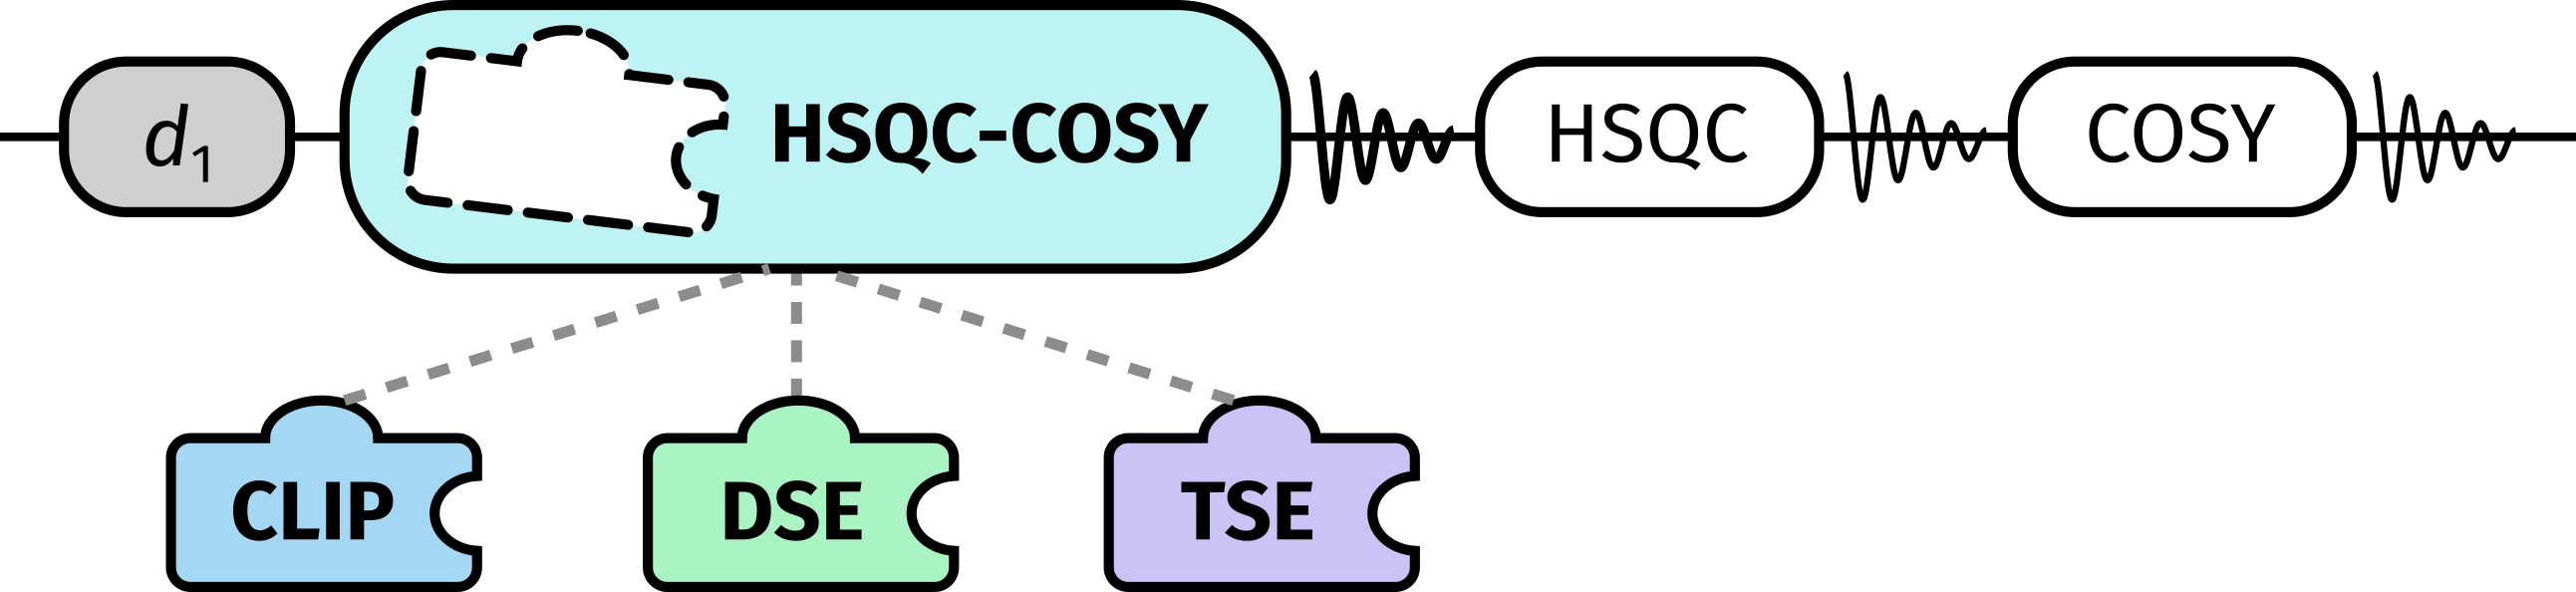
\includegraphics{toc.png}%
    \todo{TOC PIC GOES HERE}
\end{figure*}

\begin{itemize}
    \item Detailed discussion of HSQC-COSY implementations in NMR supersequences.
    \item Comparison of HSQC-COSY with HSQC-TOCSY.
    \item Sensitivity analyses of modules within typical NMR supersequences involving HSQC-COSY experiments.
\end{itemize}

NMR supersequences, as exemplified by the NOAH (NMR by Ordered Acquisition using \proton detection) technique, are a powerful way of acquiring multiple 2D data sets in much shorter durations.
This is accomplished through targeted excitation and detection of the magnetisation belonging to specific isotopologues (`magnetisation pools').
Separately, the HSQC-COSY experiment has recently seen an increase in popularity due to the high signal dispersion in the indirect dimension and the removal of ambiguity traditionally associated with HSQC-TOCSY experiments.
Here, we describe how the HSQC-COSY experiment can be integrated as a `module' within NOAH supersequences.
The benefits and drawbacks of several different pulse sequence implementations are discussed, with a particular focus on how sensitivities of other modules in the same supersequence are affected.

\clearpage

\section{Introduction}

The acceleration of multidimensional NMR spectroscopy has been an extremely popular topic in recent years, with techniques ranging from ultrafast NMR\autocite{Frydman2002PNASUSA,Pelupessy2003JACS,Frydman2003JACS} and non-uniform sampling (NUS)\autocite{Kazimierczuk2010PNMRS,Mobli2014PNMRS,Kazimierczuk2015MRC} to multiple-receiver technology\autocite{Kupce2006JACS,Kupce2008JACS,Kovacs2016MRC} and reduction of recovery delays\autocite{Kupce2007MRC,SchulzeSunninghausen2014JACS,Becker2019JMR}.
NOAH (NMR by Ordered Acquisition using \proton{} detection) experiments\autocite{Kupce2017ACIE}, which fall under the category of multiple-FID experiments\autocite{Yong2023RSCBook}, concatenate multiple 2D experiments (`modules') into a single nested pulse sequence with elision of intermediate recovery delays.
Such `supersequences' provide up to $4\times$ time savings compared to conventional, one-by-one acquisition of each 2D spectrum, and have gained popularity due to their versatility as well as the fact that they do not require specialised hardware.

Virtually all of the most commonly used 2D experiments have been adapted for use within NOAH supersequences, as neatly listed on the GENESIS website\autocite{Yong2022AC}.
In particular, we previously described the implementation of the HSQC-TOCSY module in NOAH supersequences.\autocite{Yong2021JMR}
The HSQC-TOCSY experiment is extremely information-rich, providing both `direct' responses which arise from directly bonded \CH{} pairs, and `indirect' responses from protons in the same spin system as those bound to \carbon{} \todo{(FIGURE 1A)}.
This is essentially the same information as in separate HSQC and TOCSY spectra, but with the additional benefit that the TOCSY signals are dispersed more widely across the \carbon{} indirect dimension: this serves to greatly reduce the possibility of overlap and thus increase interpretability.

One downside of the HSQC-TOCSY is the largely indiscriminate transfer of magnetisation effected by the isotropic mixing block, which means that it is difficult to determine the number of bonds separating the \carbon{} and \proton{} resonances in the `indirect' responses.
It is possible to record multiple HSQC-TOCSY spectra with different mixing times to glean insight into how many transfer steps each peak arises from.
However, this is a time-consuming process, and although multiple HSQC-TOCSY experiments could theoretically be concatenated into a NOAH supersequence, repeatedly sampling the \magn{C} magnetisation pool will lead to degraded sensitivity and reduced usefulness.

A direct method of overcoming this is to instead record an HSQC-COSY spectrum, where the `indirect' responses arise only from single-step coherence transfer between directly coupled \HH{} pairs \todo{(FIGURE 1B)}.
Experiments of this kind date back almost two decades, including the celebrated H2BC experiment\autocite{Nyberg2005JACS,Nyberg2005MRC}, and later 2BOB/H2OBC\autocite{Kupce2017MRC} and HMQC-COSY\autocite{Hu2011JBNMR}.
The 2BOB experiment in particular has previously been incorporated in NOAH supersequences\autocite{Kupce2019JMR}.
Since then, the HSQC-CLIP-COSY\autocite{Gyongyosi2018CPC,Gyongyosi2021AC} has emerged as a modern and improved experiment for this purpose: it provides pure absorption-mode lineshapes and does not suffer from amplitude modulation due to proton--proton couplings, a downside of the constant-time technique used in some of its predecessors.

Although the HSQC-CLIP-COSY performs admirably as a standalone experiment, the requirements for NOAH supersequences are more stringent: in particular, any HSQC-COSY module should---ideally---preserve unused magnetisation for later modules.
The most important example of this is the preservation of \magnnot{C} magnetisation for a later homonuclear module: an HSQC-COSY experiment in principle does not need this as it only excites \carbon{}--bound protons.
However, another key feature of the NOAH HSQC-TOCSY module is the fact that it allows for variable excitation of \magn{C} magnetisation, meaning that a portion of it can be saved for a later heteronuclear module (e.g.\ an HSQC).
We should therefore like any implementation of the HSQC-COSY to also exhibit this flexibility, as it allows the user to fine-tune the sensitivities of the modules within the supersequence for maximal performance.


\section{EVERYTHING BELOW THIS IS LIFTED FROM THESIS --- BE CAREFUL}

These often use constant-time techniques in order to remove $\nJ{HH}$ splittings and minimise linewidths in the indirect dimension; however, the drawback of this approach is that peak \textit{amplitudes} are modulated by $\nJ{HH}$.
Furthermore, it is not generally possible to obtain absorption-mode lineshapes for all peaks in the spectrum: typically the `direct' responses are in-phase absorption, and `indirect' responses antiphase dispersion.
(Here, the terms in-phase and antiphase are used with respect to $\nJ{HH}$; specifically, for the indirect peaks, this refers to the `active' coupling over which the coherence was transferred).


\section{HSQC-CLIP-COSY}

\begin{figure}[!ht]
    \centering
    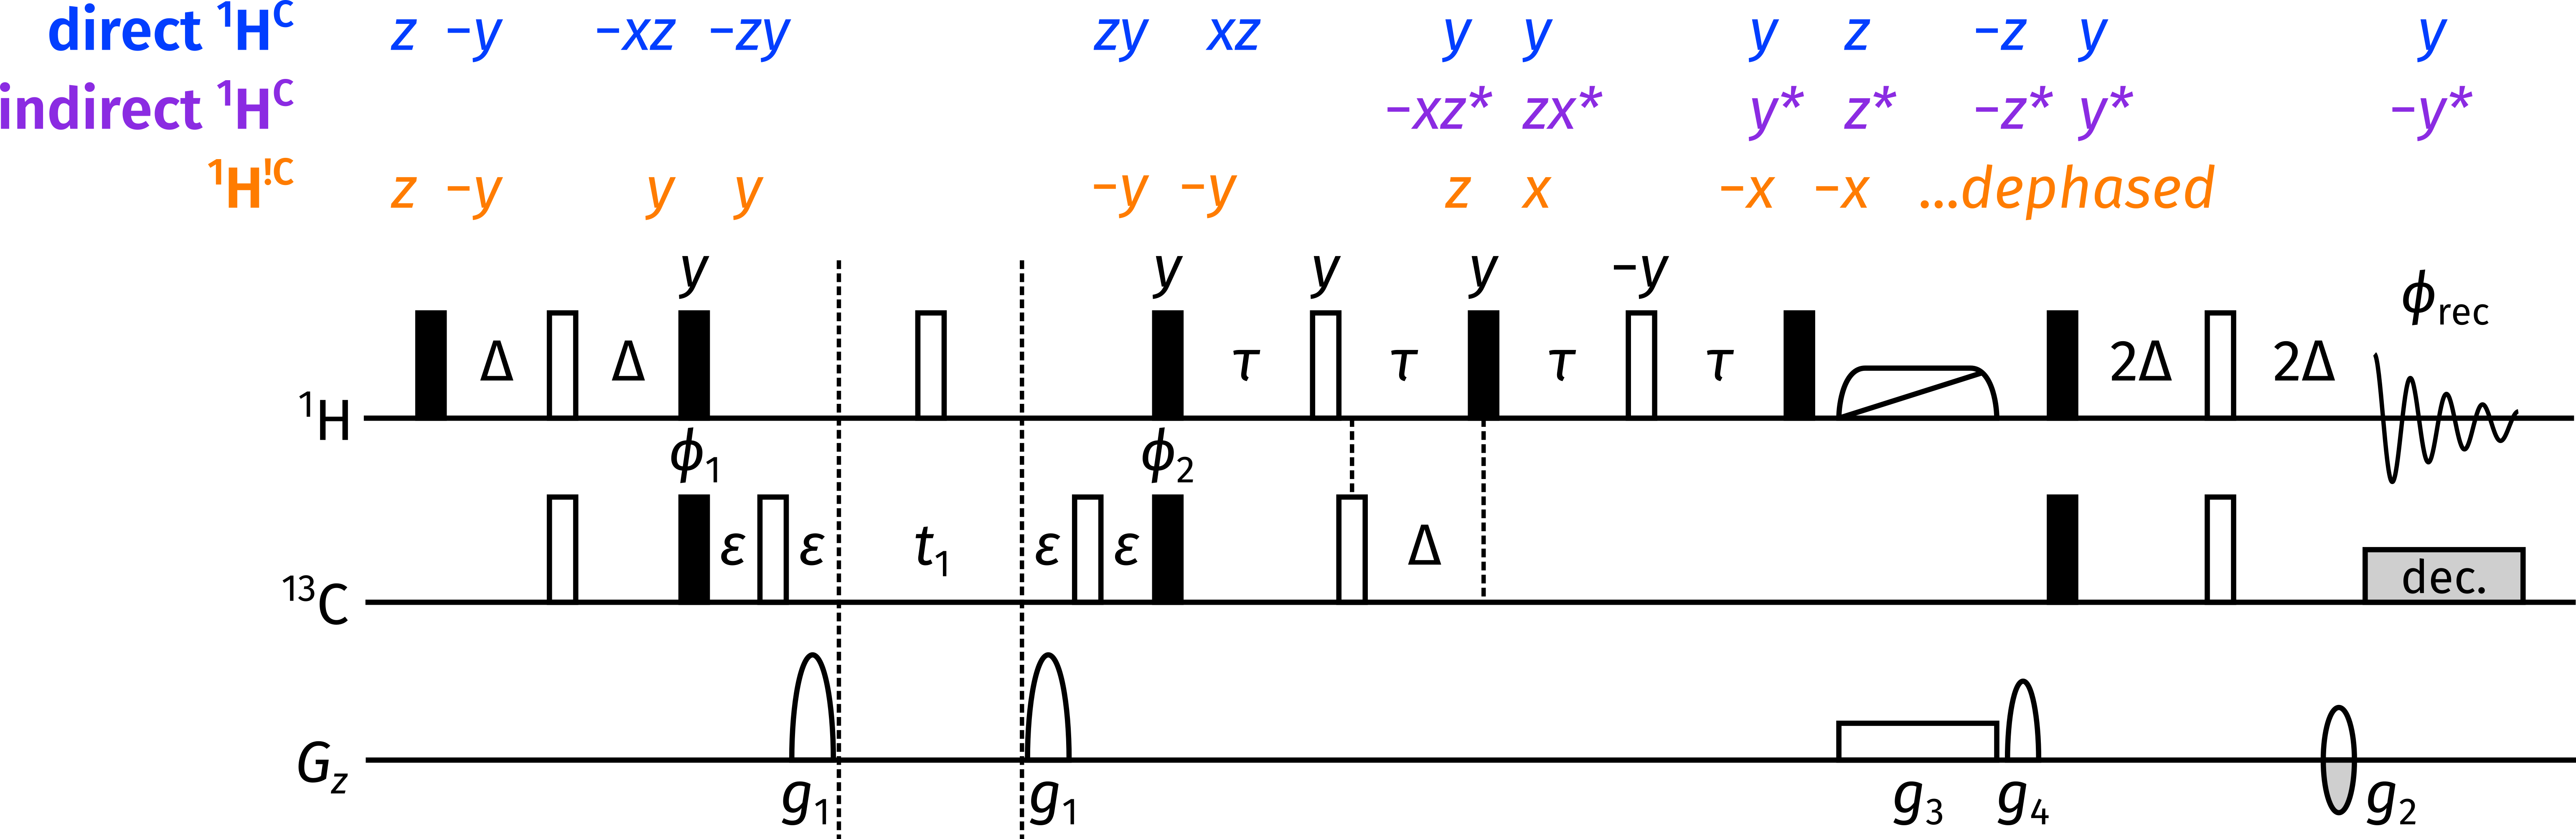
\includegraphics[]{clip_po.png}%
    \caption[HSQC-CLIP-COSY experiment]{
        HSQC-CLIP-COSY experiment with product operator analysis for the HSQC-COSY signal derived from the \magn{C} magnetisation, as well as the bulk \magnnot{C} magnetisation.
        Both the `direct', HSQC-type peaks, as well as the `indirect' responses arising from coherence transfer in the perfect echo block, are analysed.
        The shorthand notation for product operators is expanded here to deal with a three-spin $IKS$ system, where $I$ and $S$ are a mutually bonded \proton{}--\carbon{} pair as usual, and $K$ is a `remote' proton coupled to $I$.
        Terms with asterisks are on spin $K$; thus, for example, $zx*$ refers to an $I_zK_x$ term.
        The delay $\tau$ is chosen to be $1 / (4 \cdot \sum \nJ{HH})$; typically, this sum of couplings is set as \qty{30}{Hz}, leading to a value of $\tau = \qty{8.33}{\ms}$.
        The ZQF gradient $g_3$ should be calibrated as per Thrippleton et al.\autocite{Thrippleton2003ACIE}; $g_4$ is a purge gradient with arbitrary amplitude.
    }
    \label{fig:hsqcc_clip_po}
\end{figure}

These problems are circumvented by the HSQC-CLIP-COSY experiment\autocite{Gyongyosi2018CPC,Gyongyosi2021AC}, where the basic HSQC experiment is combined with clean in-phase (CLIP) coherence transfer using a perfect echo\autocite{Aguilar2012CC,Parella2019MRC,Koos2016ACIE} and ZQF\autocite{Thrippleton2003ACIE} (\cref{fig:hsqcc_clip_po}).
The use of an HSQC-type experiment means that $\nJ{HH}$ does not evolve during $t_1$, and the CLIP transfer ensures that all peaks have in-phase absorption lineshapes.
Much like the HSQC-TOCSY experiment before it, this experiment may be implemented with direct/indirect response editing: it is this version of the experiment which is shown in \cref{fig:hsqcc_clip_po}.%
\footnote{Note that this direct/indirect editing is orthogonal to \textit{multiplicity editing}, which labels both direct and indirect responses with a sign that depends on the multiplicity of the \carbon{} nucleus detected in $t_1$. The addition of multiplicity editing leads to highly confusing spectra, so is ignored here---although the option to do so \textit{is} provided in the GENESIS pulse programmes if the user so desires.}
If this editing is not desired, then the final $2\Delta$--\ang{180}($I,S$)--$2\Delta$ spin echo can simply be reduced to a minimal gradient echo, i.e.\ $\varepsilon$--\ang{180}($I$)--$\varepsilon$.

Unfortunately, the HSQC-CLIP-COSY experiment does not preserve \magnnot{C} magnetisation; thus, it cannot be directly used in a NOAH supersequence without sacrificing the sensitivity of terminal homonuclear modules.
In particular, the ZQF used in the HSQC-CLIP-COSY experiment dephases all magnetisation that is not along $z$.
If we wished to retain \magnnot{C} magnetisation, it would therefore have to (somehow) be placed along $z$ during this period, and would have to be differentiated from the HSQC-COSY signal \textit{after} the ZQF, which is not possible.%
\footnote{To be precise, although the $\oneJ{CH}$ Hamiltonian could be used to separate bulk magnetisation and the HSQC-type `direct' responses, the `indirect' responses cannot be differentiated.}
On top of that, the experiment also cannot be modified to provide partial excitation of \magn{C} magnetisation, which limits the ways in which it can be combined with other \carbon{} modules.


\section{Double spin echo HSQC-COSY}

\begin{figure}[!ht]
    \centering
    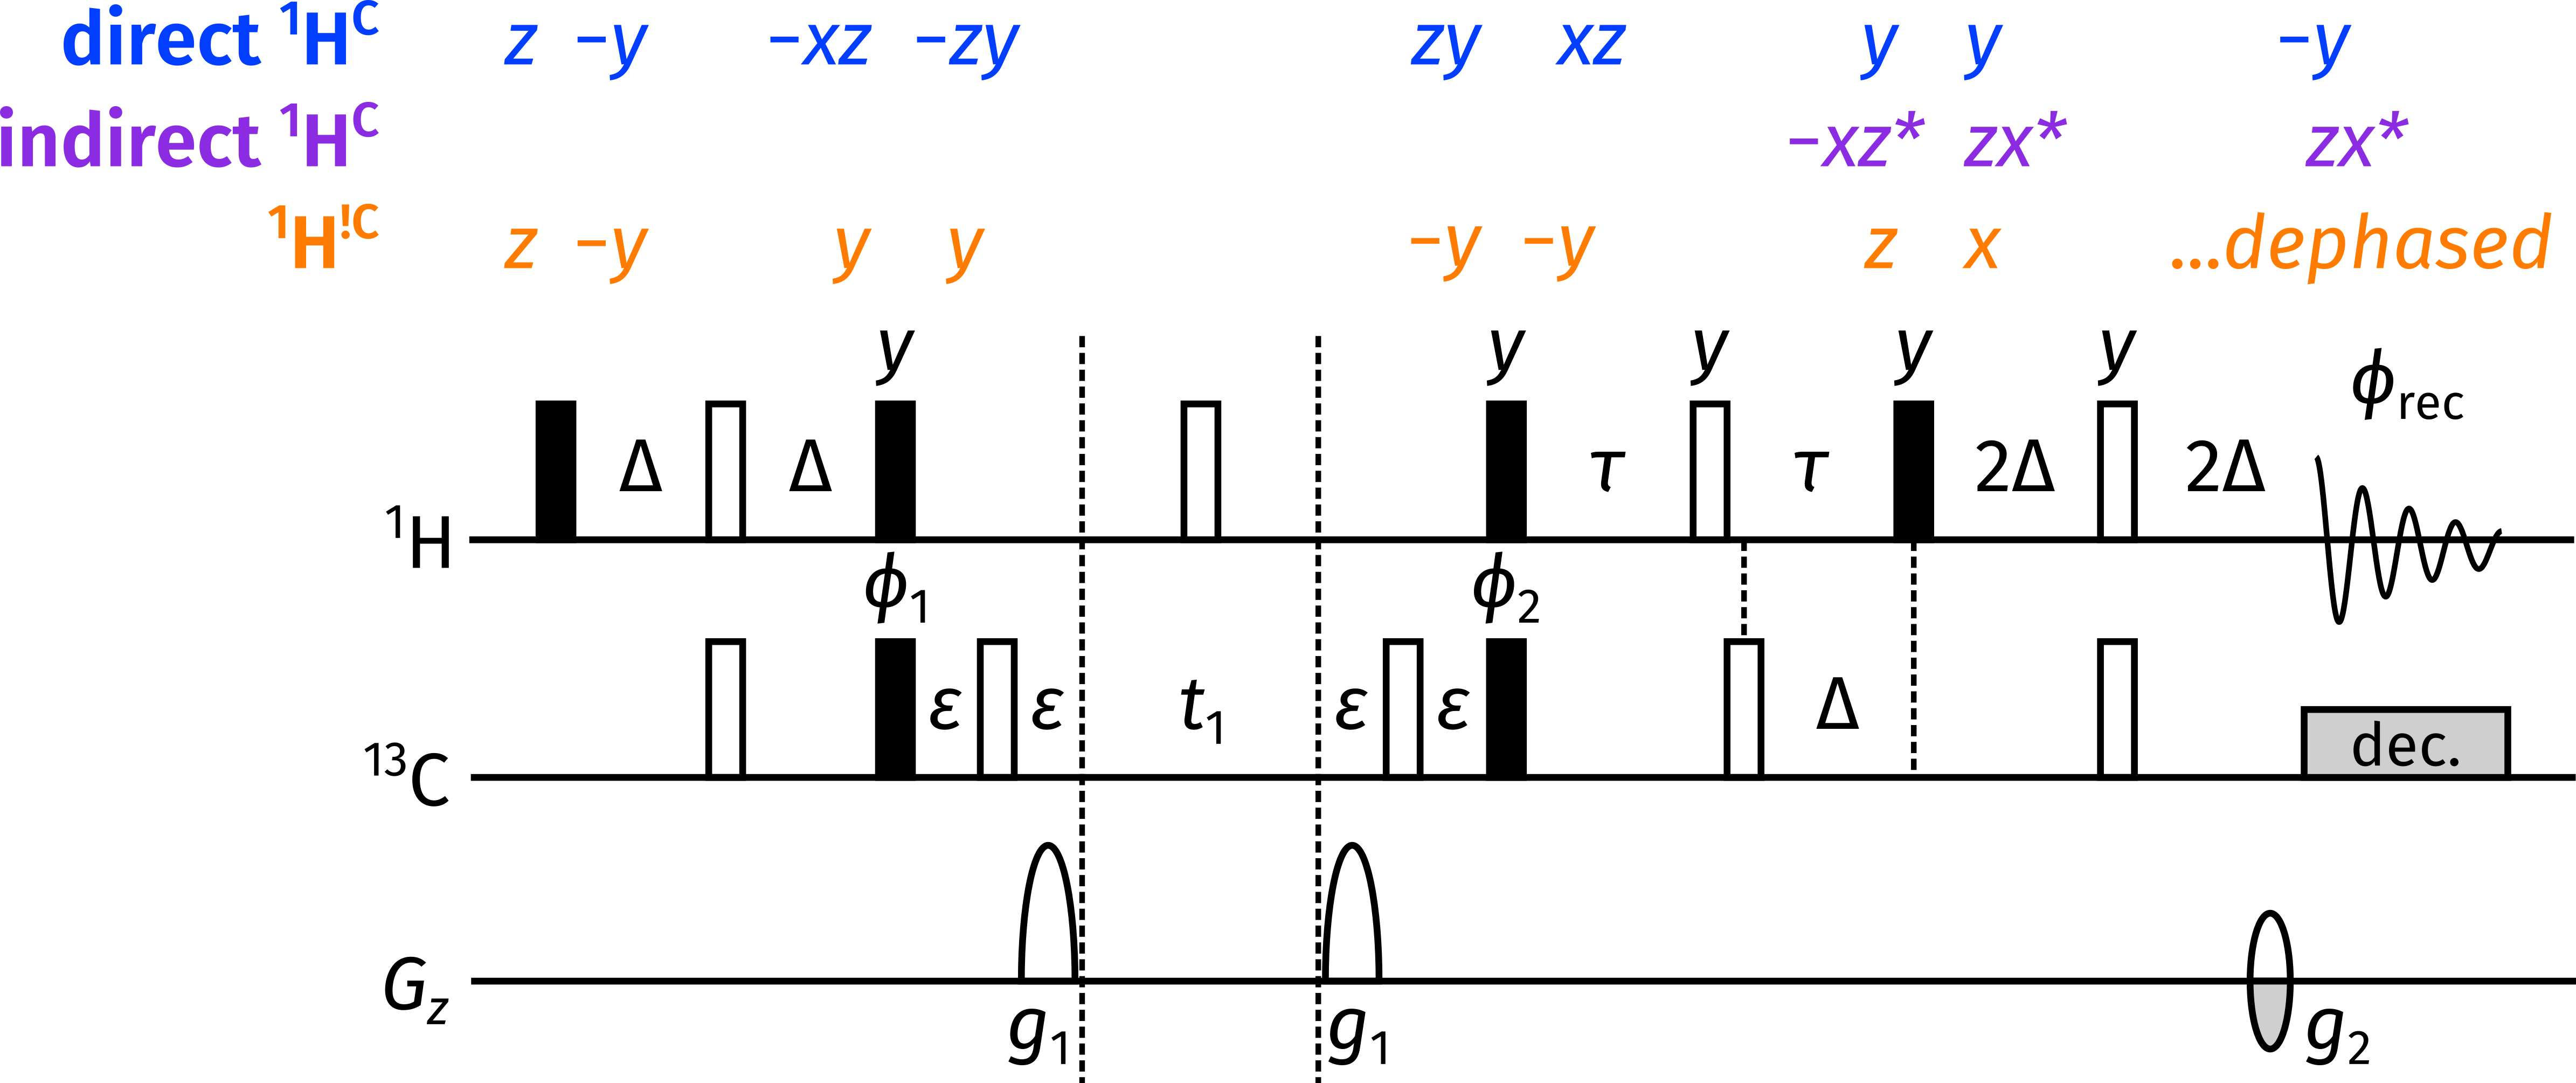
\includegraphics[]{dse_po.png}%
    \caption[Double spin echo HSQC-COSY experiment]{
        `Double spin echo' HSQC-COSY experiment; all symbols have the same meaning as in \cref{fig:hsqcc_clip_po}.
    }
    \label{fig:hsqcc_dse_po}
\end{figure}

Before tackling these problems directly, I discuss a simpler version of the HSQC-COSY experiment, which uses a simple spin echo for $\nJ{HH}$ evolution instead of the perfect echo of the CLIP version.
Together with the final $4\Delta$ spin echo, this forms a `double spin echo' (DSE) version of the HSQC-COSY experiment (\cref{fig:hsqcc_dse_po}); the `double' refers only to the mixing section after $t_1$.
The removal of the CLIP coherence transfer element leads to mixed lineshapes in this experiment, where the direct responses are (mostly) in-phase absorption, and the indirect responses (mostly) antiphase dispersion.%
\footnote{The qualifier \textit{mostly} is required because evolution of $\nJ{HH}$ during the final spin echo leads to mixtures of in-phase absorption and antiphase dispersion. This evolution is generally small, though, because $2\Delta$ is smaller than $\tau$.}

Like the CLIP version, this DSE experiment does not preserve bulk magnetisation; it is also incompatible with partial \magn{C} excitation.
However, it does provide more raw sensitivity than the CLIP version: in the CLIP version, any antiphase signal at the end of the perfect echo is destroyed by the ZQF.
All of this available signal is sampled in the DSE version, but this comes at the cost of not having pure absorption lineshapes.

It should be mentioned that prepending this DSE HSQC-COSY with the ZIP element would in fact return the bulk \magnnot{C} magnetisation to $+z$ at the end of the sequence.
However, I did not manage to test this experimentally, as my focus was on the development of the \textit{triple} spin echo HSQC-COSY below.


\section{Triple spin echo HSQC-COSY}

\begin{figure}[!ht]
    \centering
    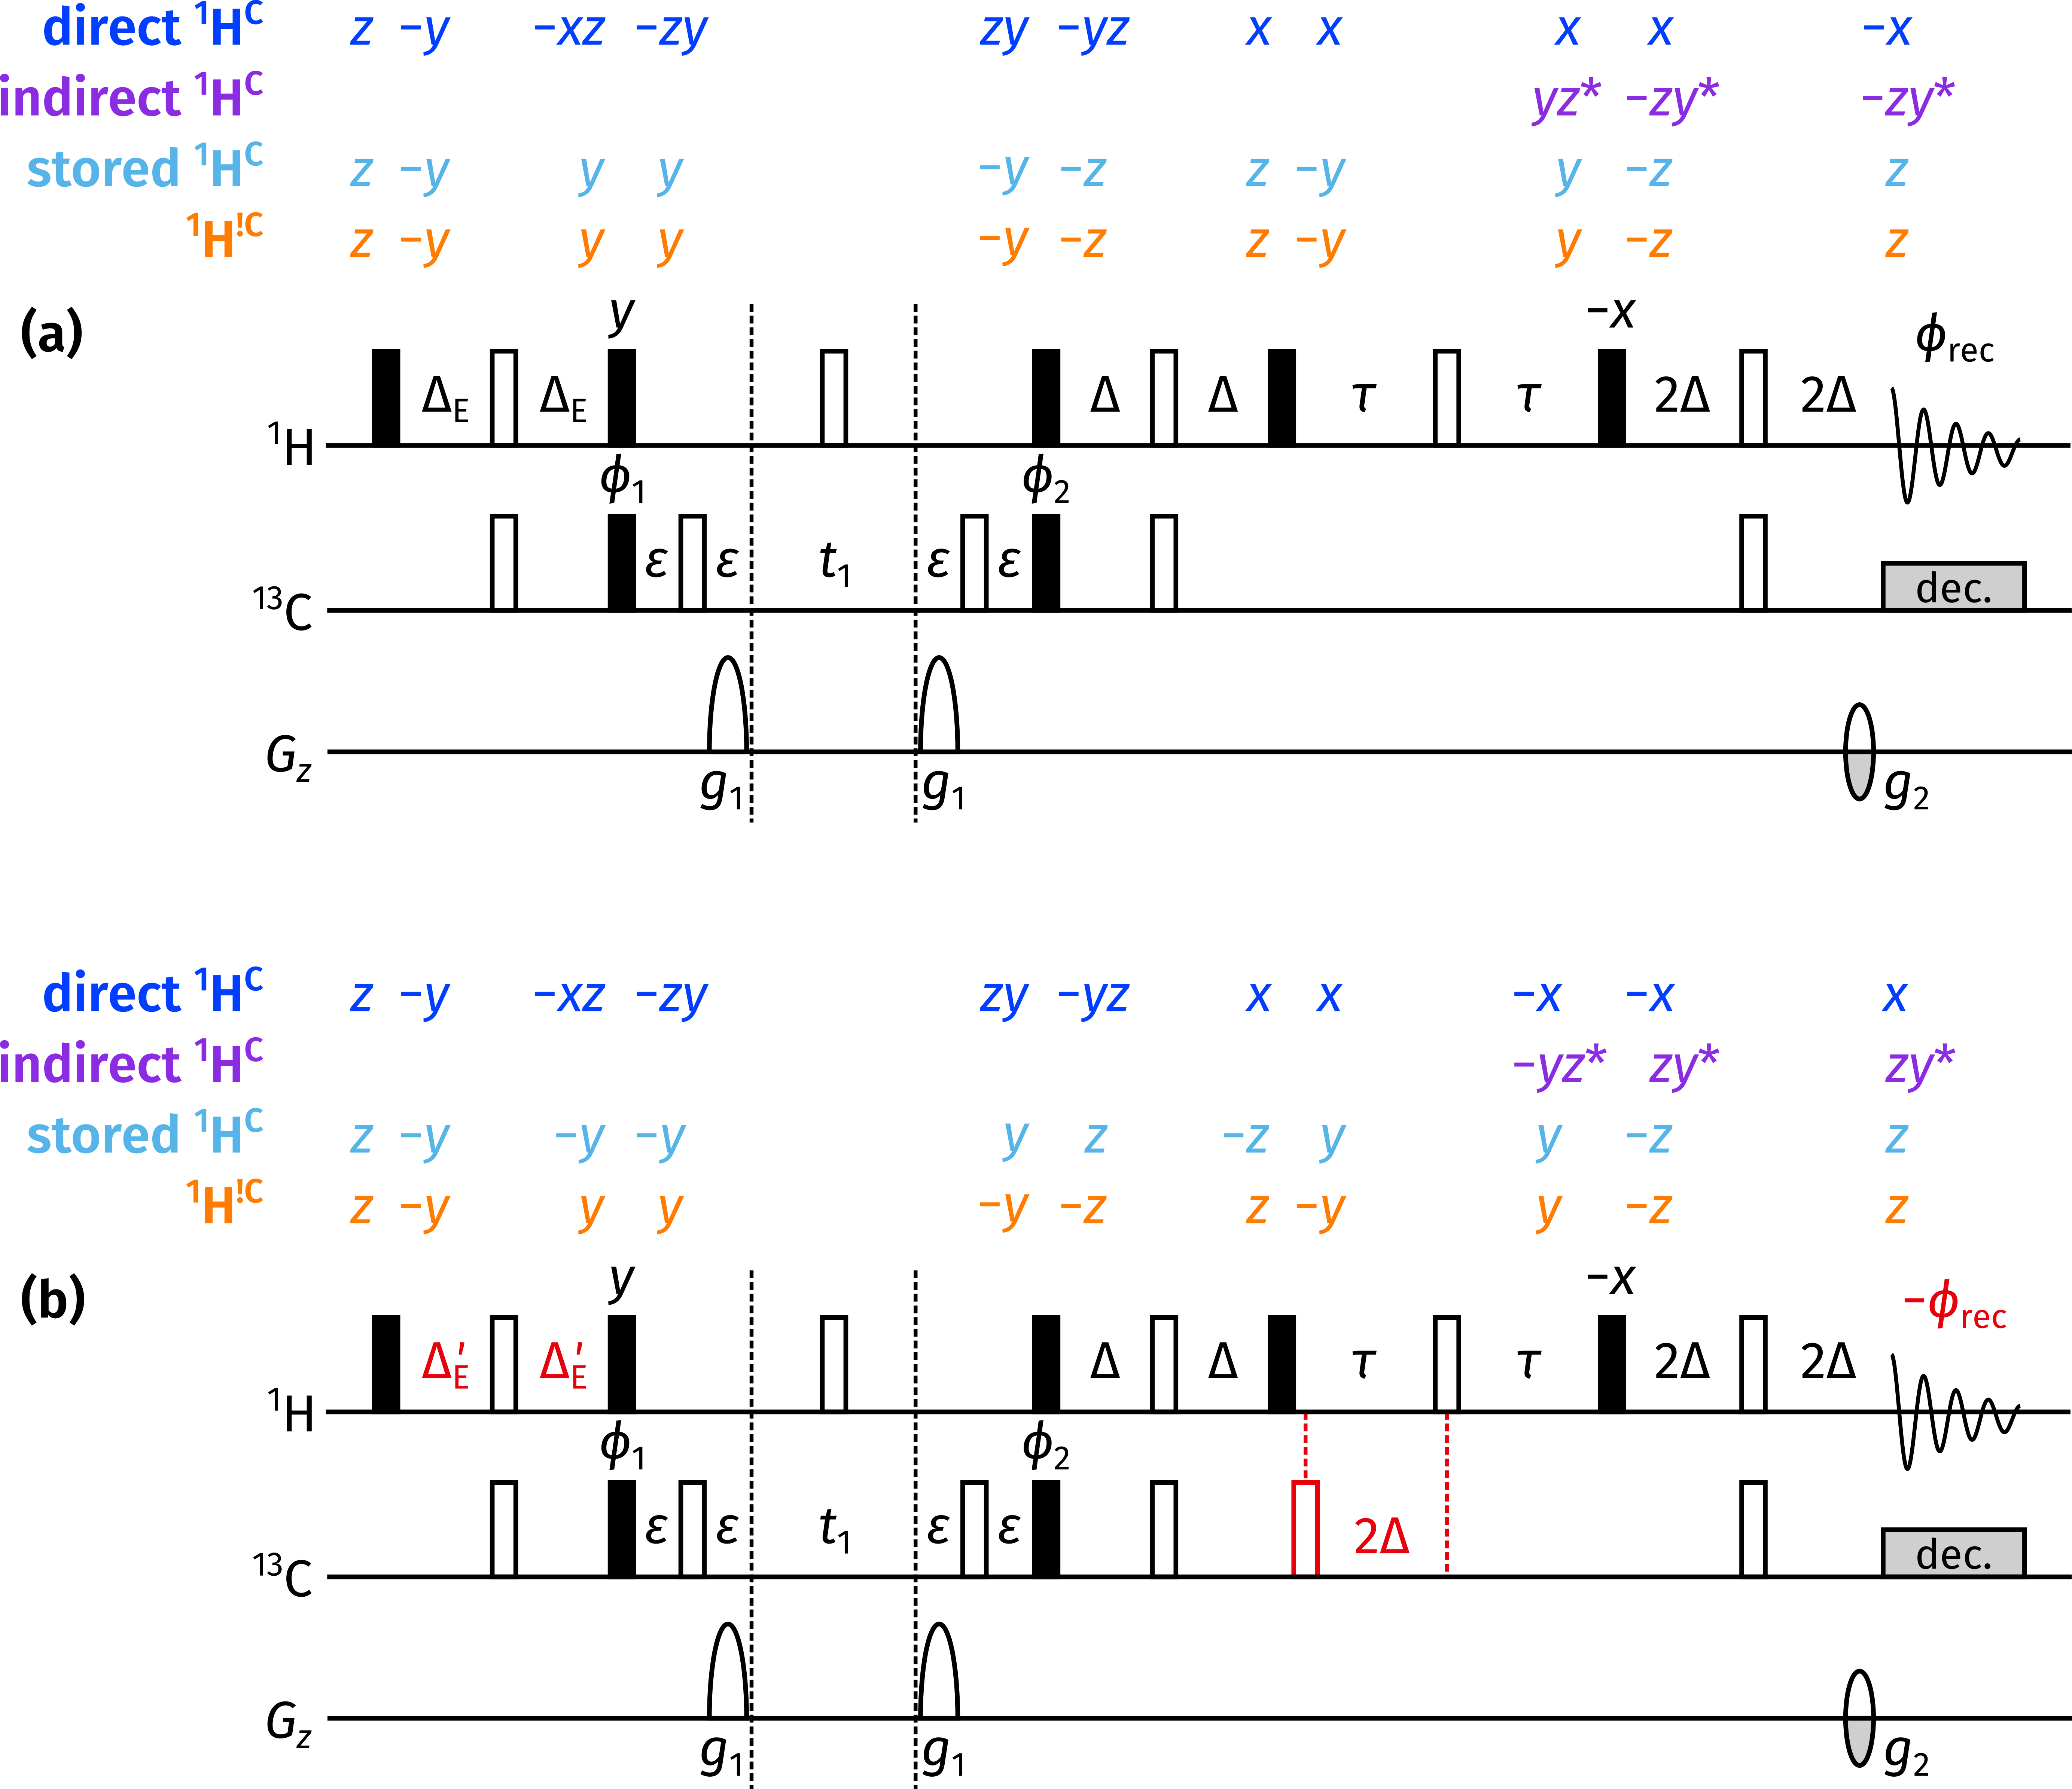
\includegraphics[]{tse_po.png}%
    {\phantomsubcaption\label{fig:hsqcc_tse_po_1}}%
    {\phantomsubcaption\label{fig:hsqcc_tse_po_2}}%
    \caption[Triple spin echo HSQC-COSY experiment]{
        `Triple spin echo' (TSE) HSQC-COSY experiment.
        \textbf{(\subref*{fig:hsqcc_tse_po_1})} The first part of the experiment; this can be used on its own, but leads to spurious `relayed' peaks arising via coherence transfer over two scalar couplings.
        \textbf{(\subref*{fig:hsqcc_tse_po_2})} The second part of the experiment; co-adding this dataset with the first part leads to suppression of the relayed peaks.
        All symbols have the same meaning as in \cref{fig:hsqcc_clip_po}.
    }
    \label{fig:hsqcc_tse_po}
\end{figure}

In the DSE HSQC-COSY, the first of the two spin echoes after $t_1$ serves a dual purpose: $\oneJ{CH}$ is allowed to evolve for a duration of $\tau - (\tau - \Delta) + \Delta = 2\Delta$ (thus generating peaks which are in-phase with respect to $\oneJ{CH}$), and $\nJ{HH}$ evolves for the total duration of $2\tau$ (allowing coherence transfer to remote spins).
The triple spin echo (TSE) HSQC-COSY is derived from the DSE version by separating the first spin echo into two distinct parts: one for $\oneJ{CH}$ refocusing, and one for $\nJ{HH}$ evolution.
As shown by the product operator analysis in \cref{fig:hsqcc_tse_po_1}, this not only preserves the bulk \magnnot{C} magnetisation, but is also compatible with partial \magn{C} excitation.

The problem with the TSE version is the spectral quality: consider an even larger spin system of the form $\ch{S-I-K-L}$, where $\{I,K,L\}$ are \proton{} and $S\/$ is \carbon{}.
At the end of $t_1$, single-quantum magnetisation on spin $I\/$ is present.
Any evolution of $J_{IK}$ in the first spin echo (of duration $2\Delta$) leads to terms of the form $2I_yK_z$, and can then be transferred onto spin $K\/$ by the subsequent \angang{90}{x} pulse.
This magnetisation can then further evolve under $J_{KL}$ during the $2\tau$ spin echo, and then be transferred a \textit{second} time by the \angang{90}{-x} pulse to spin $L$.
Since the intensity of this transfer pathway is proportional to $\sin(2\cpi J_{IK}\Delta)$, these `relay' artefacts are especially prominent for large $J_{IK}$.

In order to suppress these, the experiment must be run a second time but with an additional \ang{180} \carbon{} pulse inserted during the second spin echo (\cref{fig:hsqcc_tse_po_2}).%
\footnote{A very similar strategy is used in the Bruker seHSQC pulse sequence \texttt{hsqcedetgpsisp2.4} to suppress the COSY-type artefacts. However, to the best of my knowledge, this sequence has not been published anywhere.}
Any magnetisation still on spin $I\/$ will therefore evolve under $\oneJ{CH}$ for a total period of $4\Delta$, leading to net inversion.
However, magnetisation which has already been transferred to spin $K\/$ at this point will not be inverted: it is this magnetisation which is responsible for the relay artefacts.
Therefore, by subtracting the two datasets (or equivalently, inverting the receiver phase and adding the two datasets), the desired peaks will be added up and the artefacts cancelled through subtraction.

The insertion of this \ang{180} pulse also causes any unexcited \magn{C} magnetisation to be inverted.
In order to ensure that this is returned to $+z$ at the end of the sequence (and not $-z$), the initial INEPT delay must be \textit{lengthened} instead of shortened, as per:
\begin{equation}
    \label{eq:delta_e_prime}
    \DeltaE' = \frac{2\Delta (\cpi - \arcsin f)}{\cpi},
\end{equation}
where, as before, $f\/$ is the proportion of magnetisation to be excited.


\section{Supersequences}

\begin{figure}[!htp]
    \centering
    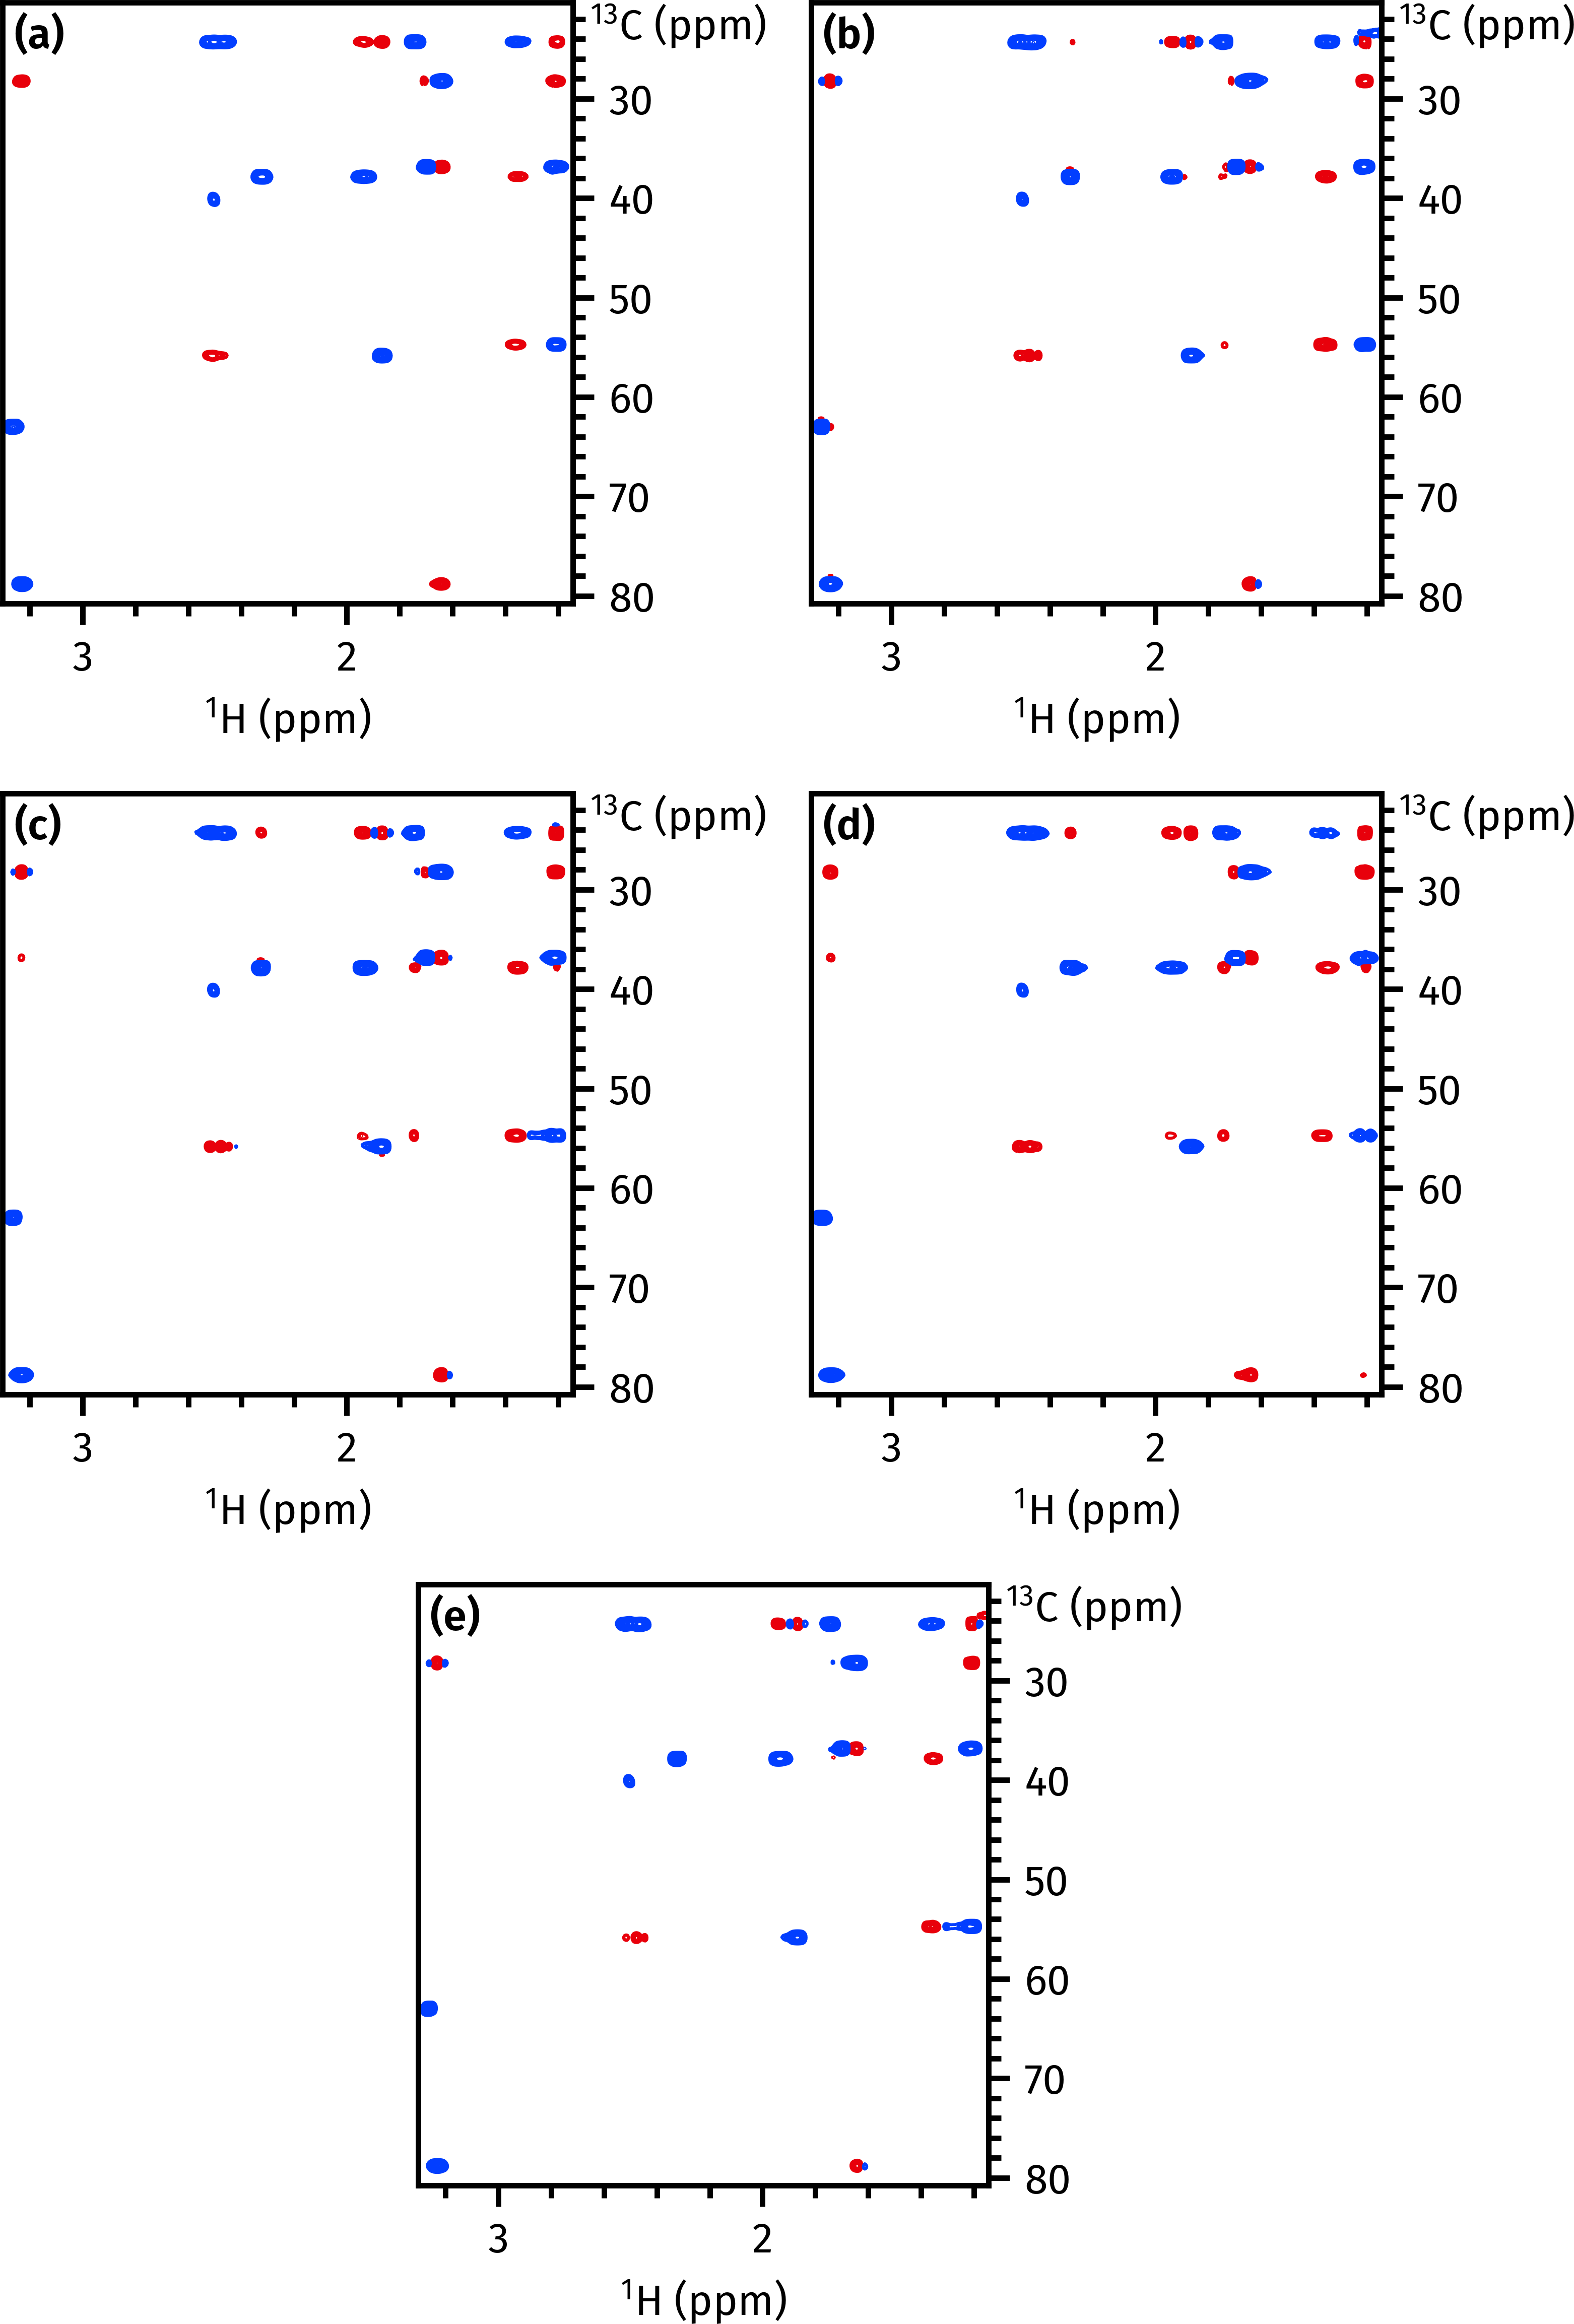
\includegraphics[]{hsqccosy_comp.png}%
    {\phantomsubcaption\label{fig:hsqccosy_comp_clip}}%
    {\phantomsubcaption\label{fig:hsqccosy_comp_dse}}%
    {\phantomsubcaption\label{fig:hsqccosy_comp_tse_norps}}%
    {\phantomsubcaption\label{fig:hsqccosy_comp_tocsy}}%
    {\phantomsubcaption\label{fig:hsqccosy_comp_tse}}%
    \caption[Comparison of spectra acquired with different HSQC-COSY modules]{
        HSQC-COSY and HSQC-TOCSY spectra, taken from (respectively) \noah{Sc,S,Cc} and \noah{St,S,Cc} experiments.
        \textbf{(\subref*{fig:hsqccosy_comp_clip})} HSQC-CLIP-COSY.
        \textbf{(\subref*{fig:hsqccosy_comp_dse})} DSE HSQC-COSY.
        \textbf{(\subref*{fig:hsqccosy_comp_tse_norps})} TSE HSQC-COSY without suppression of relay artefacts (described in the text).
        \textbf{(\subref*{fig:hsqccosy_comp_tocsy})} HSQC-TOCSY with \qty{10}{\ms} mixing time.
        \textbf{(\subref*{fig:hsqccosy_comp_tse})} TSE HSQC-COSY with suppression of relay artefacts.
        7A-210303
    }
    \label{fig:hsqccosy_comp}
\end{figure}

\begin{figure}[!ht]
    \centering
    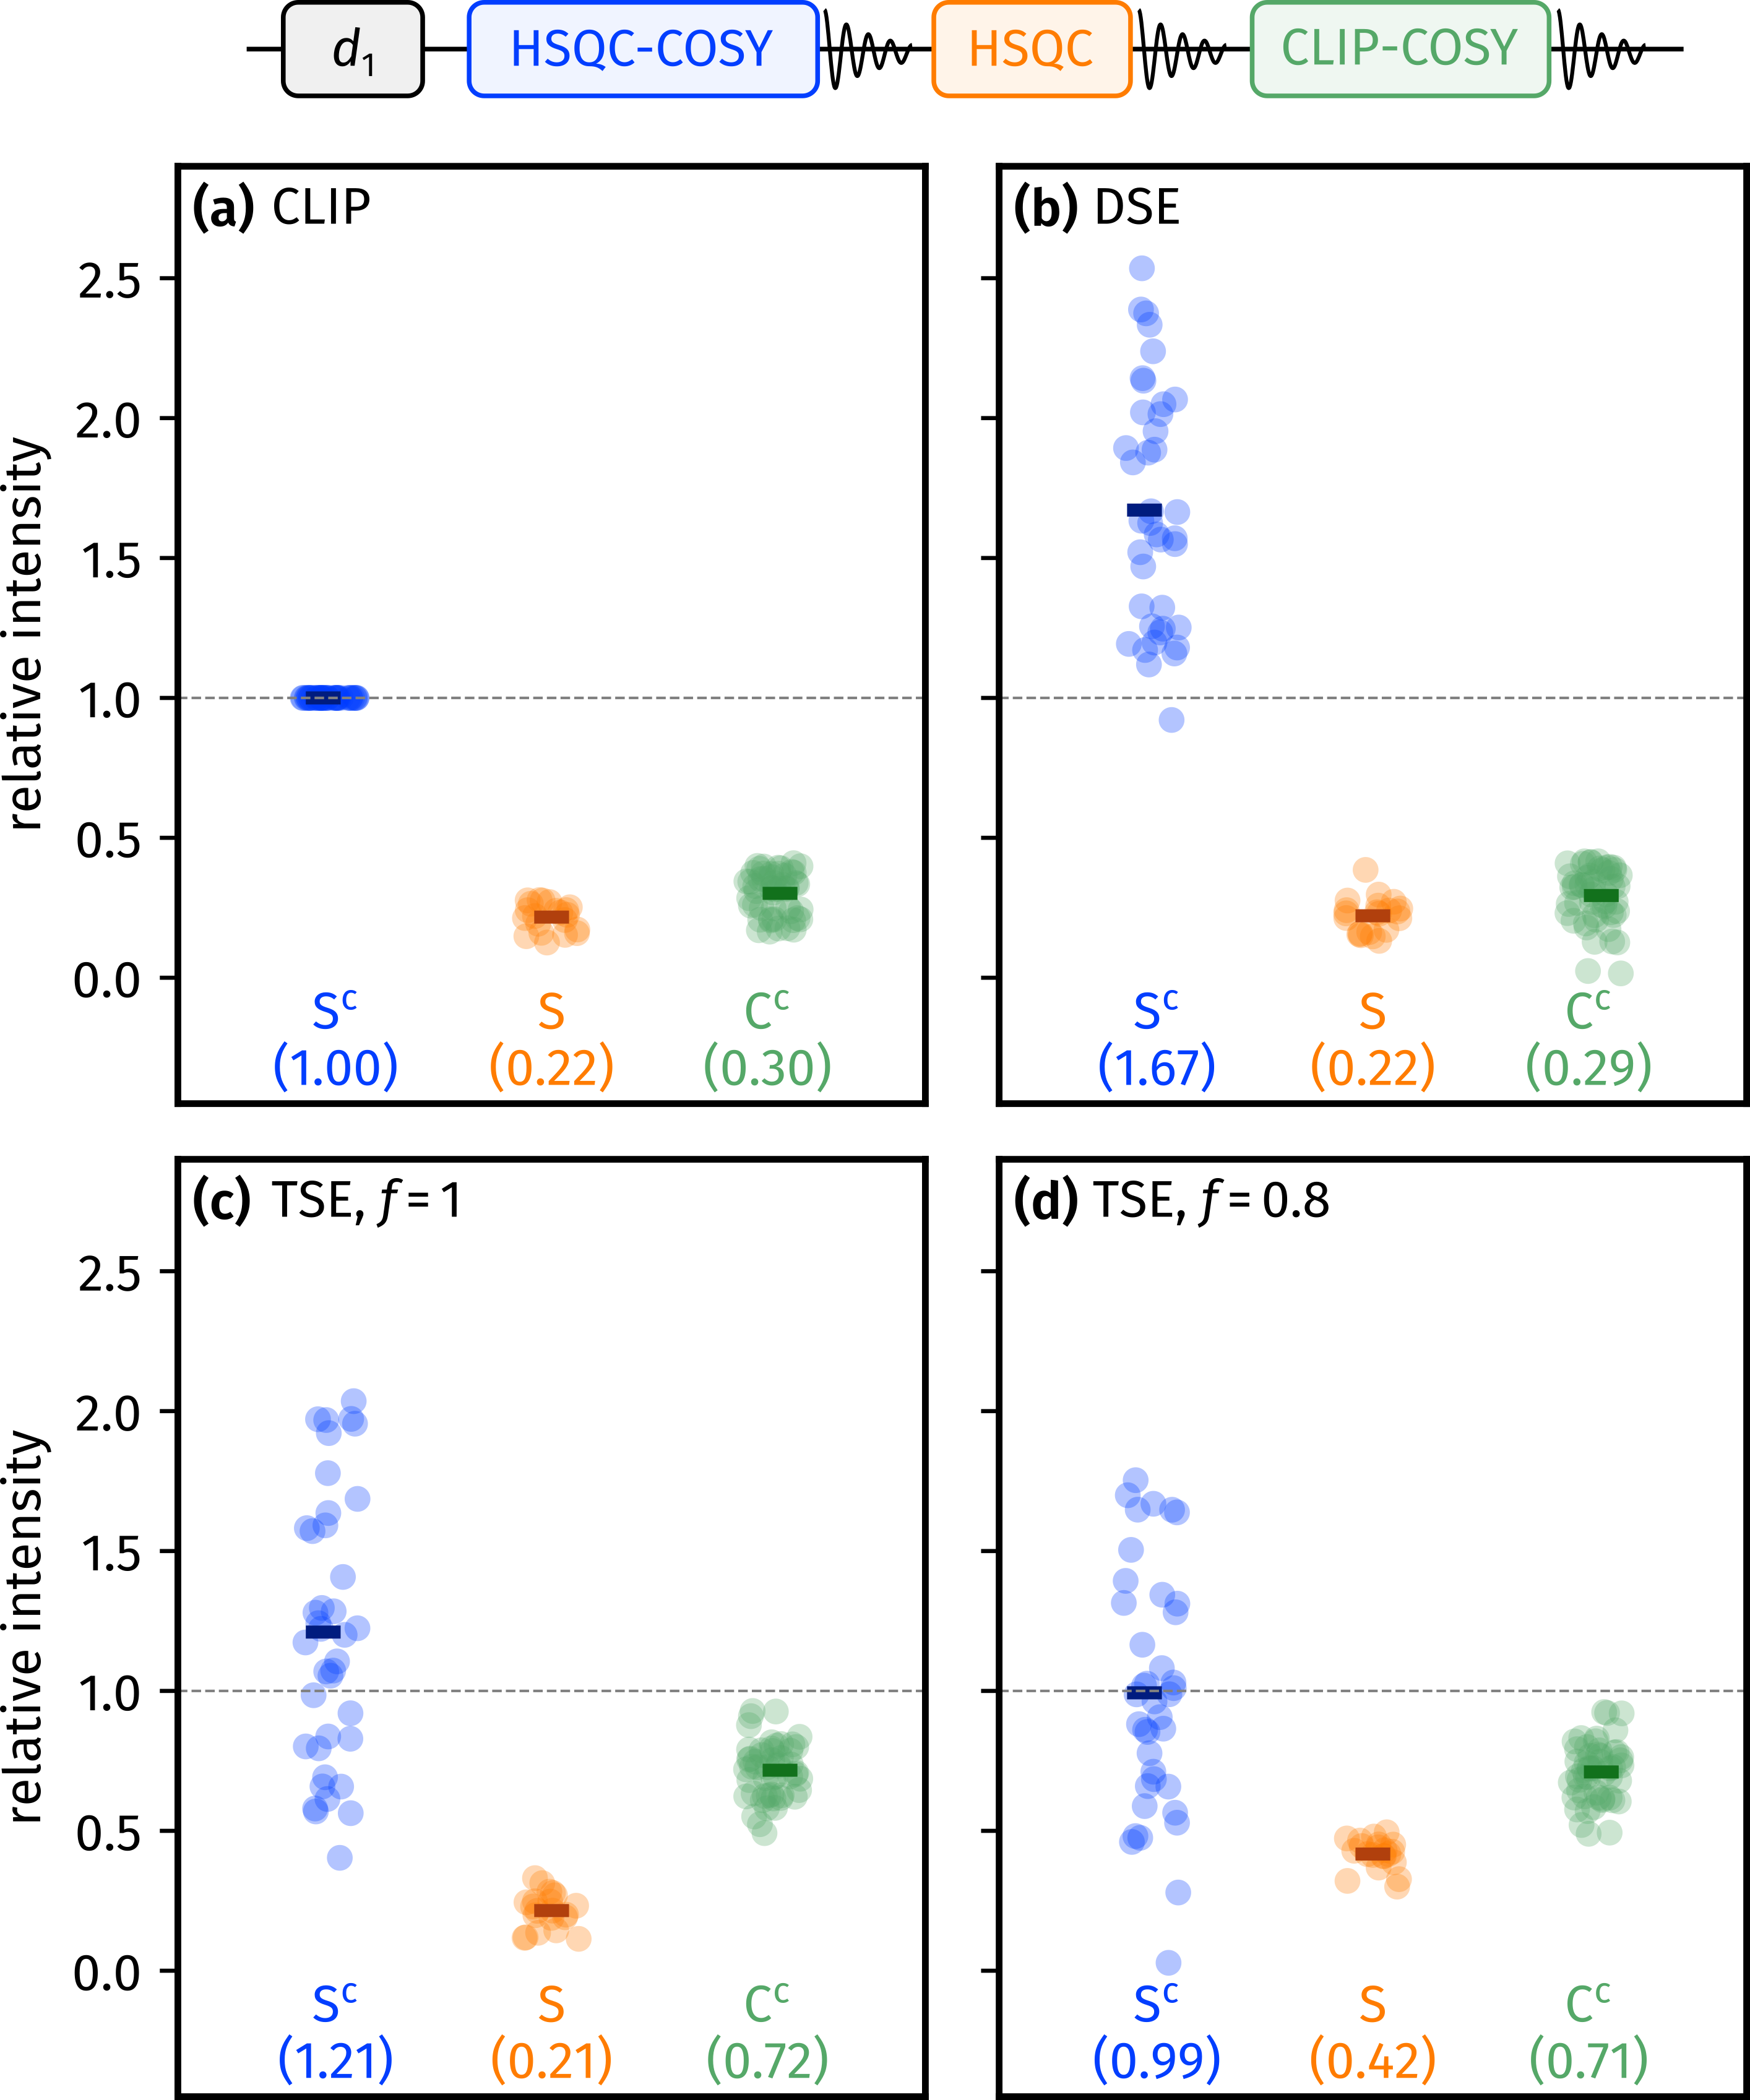
\includegraphics[]{hsqccosy_sens.png}%
    {\phantomsubcaption\label{fig:hsqccosy_sens_clip}}%
    {\phantomsubcaption\label{fig:hsqccosy_sens_dse}}%
    {\phantomsubcaption\label{fig:hsqccosy_sens_tse_1}}%
    {\phantomsubcaption\label{fig:hsqccosy_sens_tse_0p8}}%
    \caption[Sensitivity comparisons for \noah{Sc,S,Cc} supersequences]{
        Sensitivity comparisons for all three modules in \noah{Sc,S,Cc} supersequences.
        Peak intensities are relative to the HSQC-CLIP-COSY module itself (the leftmost column in (\subref*{fig:hsqccosy_sens_clip})), as well as HSQC and CLIP-COSY spectra from a \noah{S,Cc} experiment.
        Numbers in parentheses indicate averages over all peaks.
        \textbf{(\subref*{fig:hsqccosy_sens_clip})} HSQC-CLIP-COSY.
        \textbf{(\subref*{fig:hsqccosy_sens_dse})} DSE HSQC-COSY.
        \textbf{(\subref*{fig:hsqccosy_sens_tse_1})} TSE HSQC-COSY, acquired with $f = 1$.
        \textbf{(\subref*{fig:hsqccosy_sens_tse_0p8})} TSE HSQC-COSY, acquired with $f = 0.8$.
        7A-210723
    }
    \label{fig:hsqccosy_sens}
\end{figure}

The spectral quality, and sensitivity, of all of these modules is captured in \cref{fig:hsqccosy_comp,fig:hsqccosy_sens}.
The CLIP version (\cref{fig:hsqccosy_comp_clip,fig:hsqccosy_sens_clip}) has the best lineshapes, but its sensitivity is slightly lower.
The DSE version (\cref{fig:hsqccosy_comp_dse,fig:hsqccosy_sens_dse}) provides greater sensitivity, but at the cost of impure lineshapes.

For the TSE version, we first look at the importance of the relay artefact suppression procedure described above.
The extra relay artefacts are clearly visible in \cref{fig:hsqccosy_comp_tse_norps}, acquired using the `basic' sequence in \cref{fig:hsqcc_tse_po_1} only.
(As previously mentioned, these arise from large $\nJ{HH}$ which evolve during the $2\Delta$ spin echo; for this specific compound, the offending couplings are $^3\!J\/$ between two axial protons in a six-membered ring, and $^2\!J\/$ in diastereotopic methylenes).
The presence of these peaks largely defeats the purpose of using an HSQC-COSY experiment; in fact, this unoptimised TSE HSQC-COSY is qualitatively very similar to an HSQC-TOCSY acquired with a short mixing time of \qty{10}{\ms} (\cref{fig:hsqccosy_comp_tocsy}).%
\footnote{The HSQC-TOCSY even gives better peak shapes, since the DIPSI mixing transfers in-phase magnetisation to in-phase magnetisation.}
However, these artefacts can be efficiently removed using the suppression technique described in the text above; the result in \cref{fig:hsqccosy_comp_tse} is qualitatively similar to the two other HSQC-COSY experiments.
Using this suppression technique, the sensitivity of the TSE HSQC-COSY (when acquired with $f = 1$) falls between that of the CLIP and DSE versions.

\Cref{fig:hsqccosy_sens} also shows the relative sensitivities of the later modules in \noah{Sc,S,Cc} supersequences.
In all of the first three cases (CLIP, DSE, and TSE HSQC-COSY with $f = 1$, \cref{fig:hsqccosy_sens_clip,fig:hsqccosy_sens_dse,fig:hsqccosy_sens_tse_1}), the HSQC sensitivity is low (ca.\ 20\%) because no \magn{C} magnetisation is retained for it to use.
Thus, the signal derives only from \magn{C} magnetisation which has recovered during the HSQC-COSY FID.
However, when the TSE version is used, partial \magn{C} excitation can be used to control this sensitivity: for example, when $f = 0.8$ (\cref{fig:hsqccosy_sens_tse_0p8}), the HSQC-COSY sensitivity is decreased (on average equalling that of the HSQC-CLIP-COSY), but the sensitivity of the HSQC module is almost doubled.
Generally, choosing a value of $f < 1$ allows for the HSQC-COSY and HSQC sensitivities to be better balanced.

Finally, the CLIP-COSY module suffers when the HSQC-CLIP-COSY or the DSE HSQC-COSY are used, because both of these dephase \magnnot{C} magnetisation;
however, the TSE version successfully preserves around $70\%$ of this magnetisation for it, regardless of the value of $f$.
(This value is slightly lower than the approximately $90\%$ magnetisation preserved by the HSQC module, because the bulk magnetisation is placed in the transverse plane during the $2\tau$ spin echo (\cref{fig:hsqcc_tse_po_1}) and experiences losses due to $\nJ{HH}$ evolution.)


\section{HSQC-COSY in context}

\begin{figure}[!ht]
    \centering
    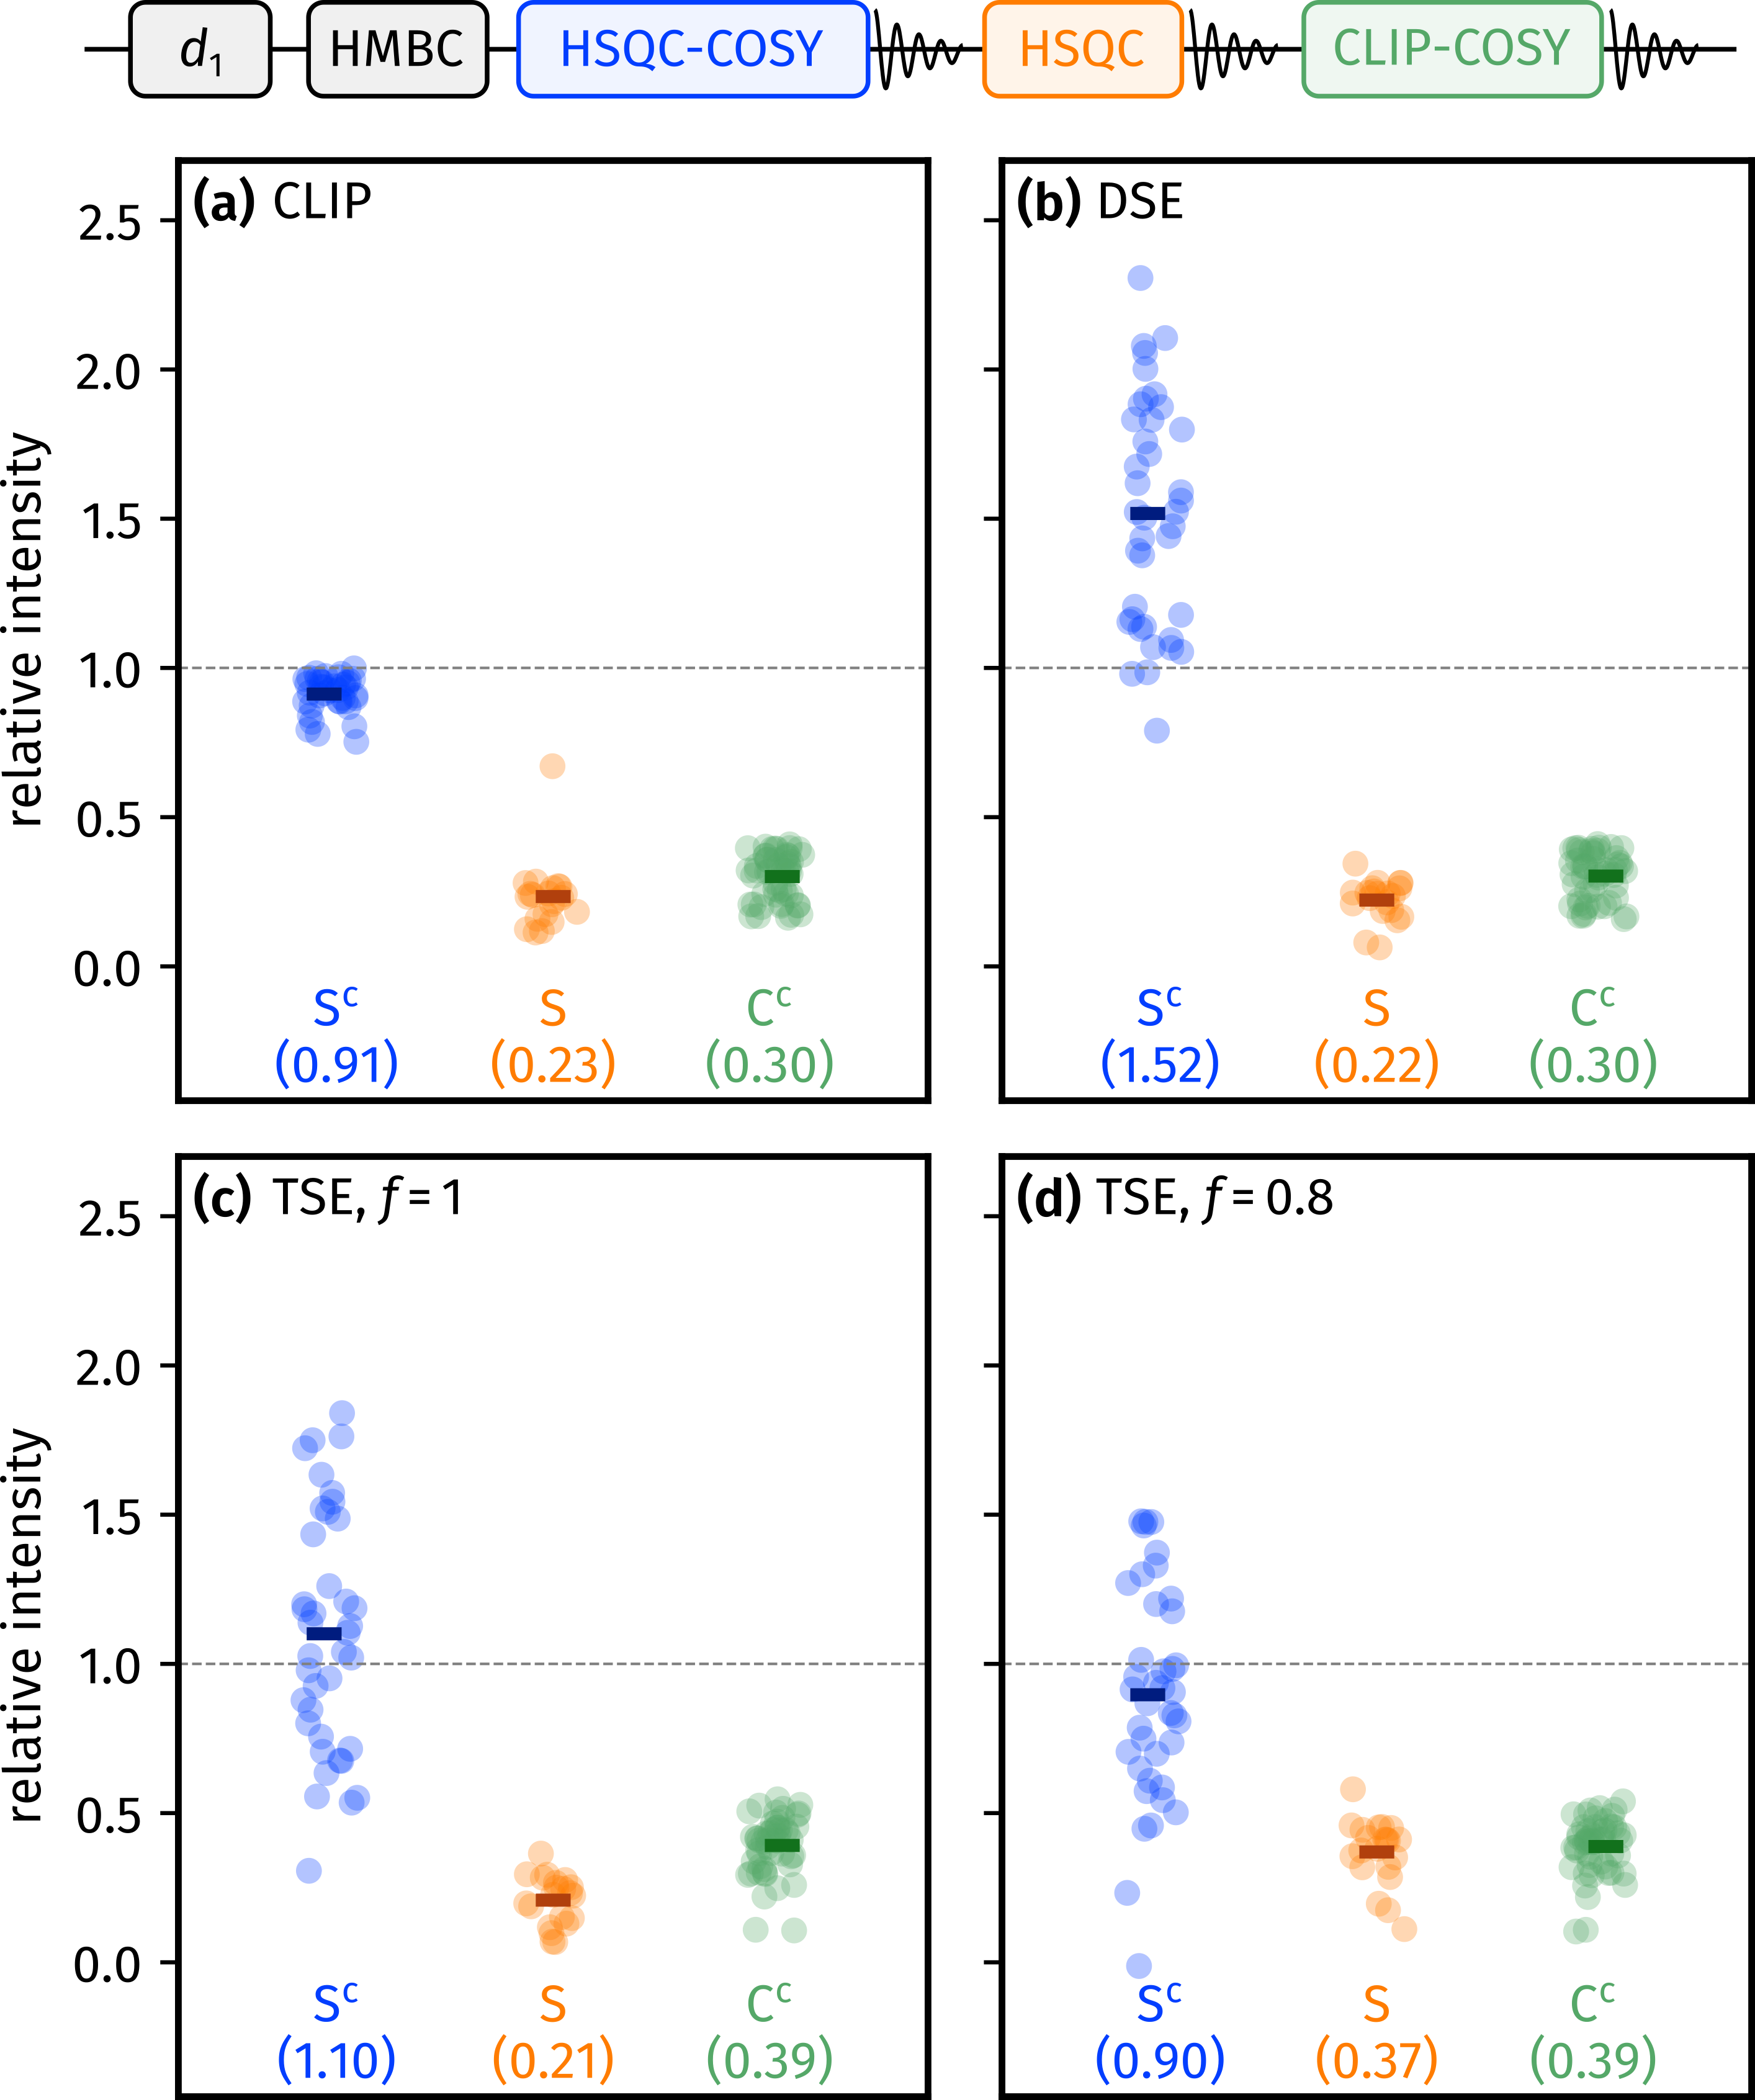
\includegraphics[]{hsqccosy_sens_with_hmbc.png}%
    {\phantomsubcaption\label{fig:hsqccosy_sens_with_hmbc_clip}}%
    {\phantomsubcaption\label{fig:hsqccosy_sens_with_hmbc_dse}}%
    {\phantomsubcaption\label{fig:hsqccosy_sens_with_hmbc_tse_1}}%
    {\phantomsubcaption\label{fig:hsqccosy_sens_with_hmbc_tse_0p8}}%
    \caption[Sensitivity comparisons for \noah{B,Sc,S,Cc} supersequences]{
        Sensitivity comparisons for the three last modules in \noah{B,Sc,S,Cc} supersequences.
        Peak intensities are relative to the HSQC-CLIP-COSY module from a \noah{Sc,S,Cc} supersequence, and HSQC and CLIP-COSY spectra from a \noah{S,Cc} experiment (these are the same reference spectra as used in \cref{fig:hsqccosy_sens}).
        Numbers in parentheses indicate averages over all peaks.
        \textbf{(\subref*{fig:hsqccosy_sens_with_hmbc_clip})} HSQC-CLIP-COSY.
        \textbf{(\subref*{fig:hsqccosy_sens_with_hmbc_dse})} DSE HSQC-COSY.
        \textbf{(\subref*{fig:hsqccosy_sens_with_hmbc_tse_1})} TSE HSQC-COSY, acquired with $f = 1$.
        \textbf{(\subref*{fig:hsqccosy_sens_with_hmbc_tse_0p8})} TSE HSQC-COSY, acquired with $f = 0.8$.
        7A-210723
    }
    \label{fig:hsqccosy_sens_with_hmbc}
\end{figure}

In \noah{Sc,S,Cc}-type supersequences, using the TSE HSQC-COSY module here appears to be a sensible option as it is capable of preserving some \magn{C} magnetisation for the HSQC, as well as all \magnnot{C} magnetisation for the CLIP-COSY.
However, this may not necessarily be so important in the context of a larger supersequence---particularly one which begins with the HMBC module, which \textit{already} dephases \magnnot{C} magnetisation (meaning that there is not much of it to preserve).

\Cref{fig:hsqccosy_sens_with_hmbc} provides the same sensitivity comparisons as in \cref{fig:hsqccosy_sens}, but in the context of a \noah{B,Sc,S,Cc} supersequence instead.
The HSQC-COSY and HSQC modules largely follow the same pattern as before, but with an approximate 10\% loss across the board: this reflects the imperfect preservation of \magn{C} magnetisation by the $zz$-HMBC module.
The CLIP-COSY module, however, has a substantially lower sensitivity regardless of which HSQC-COSY module is chosen.
When the CLIP or DSE HSQC-COSY modules are used, the CLIP-COSY retains only roughly 30\% of its original intensity: this is the same as in \cref{fig:hsqccosy_sens}.
With the TSE HSQC-COSY, this is boosted to around 40\% because there is one extra FID in which the \magnnot{C} polarisation can be recovered.
However, the use of the HMBC module at the beginning effectively places an upper limit on the amount of signal available to this module.

For virtually all homonuclear modules (including the CLIP-COSY), this small difference in sensitivity will not make a real difference in the interpretability of the spectrum.
This is especially so considering that the HMBC module---which has a far lower sensitivity---is also present in the supersequence:
a CLIP-COSY with 30\% of its original sensitivity is still more intense than the HMBC experiment.
This argument was used in justifying the \noah{B,S,Cc} experiment, and logically, should be equally applicable to the \noah{B,Sc,S,Cc} experiment.
In this case, the only compelling reason to use the TSE HSQC-COSY would be to preserve a portion of \magn{C} magnetisation for a later \carbon{} module.
Thus, in this context, the decision of which HSQC-COSY module to use is slightly more nuanced: the cleaner lineshapes provided by the CLIP version, or the sensitivity of the DSE version, may be more preferable.


\section*{Acknowledgements}

We thank Dr Mohammadali Foroozandeh (University of Oxford) for helpful discussions.
\meshort{}\ thanks the Clarendon Fund (University of Oxford) and the EPSRC Centre for Doctoral Training in Synthesis for Biology and Medicine (EP/L015838/1) for a studentship, generously supported by AstraZeneca, Diamond Light Source, Defence Science and Technology Laboratory, Evotec, GlaxoSmithKline, Janssen, Novartis, Pfizer, Syngenta, Takeda, UCB, and Vertex.

% Fakesection Bibliography
\AtNextBibliography{\small}
\printbibliography{}
\end{refsection}


% Fakesection ================= SI ==================

\clearpage
\begin{refsection}
\newcommand{\sectionbreak}{\clearpage}
\renewcommand*{\thefigure}{S\arabic{figure}}
\renewcommand*{\thesection}{S\arabic{section}}
\renewcommand*{\thetable}{S\arabic{table}}
\renewcommand*{\thepage}{S\arabic{page}}
\setcounter{page}{1}
\setcounter{figure}{0}
\setcounter{section}{0}
\setcounter{table}{0}
\onehalfspacing

\hspace{0pt}
\vfill
\begin{center}
    \huge
    Supporting Information

    \vspace{0.3cm}

    \textit{for}

    \vspace{0.3cm}

    \articletitle{}

    \vspace{0.6cm}

    \Large \me{},\textsuperscript{1} \eriks{},\textsuperscript{2} \tim{}\textsuperscript{1,\texttt{*}}

    \vspace{0.6cm}

    \large \textsuperscript{1} \textit{\crl{}}

    \textsuperscript{2} \textit{\brukeruk{}}

    \textsuperscript{\texttt{*}} \texttt{tim.claridge@chem.ox.ac.uk}

\end{center}
\vfill

\newpage
\section*{Contents}

\startcontents[si]
\printcontents[si]{ }{1}{}
\vfill
\hspace{0pt}
\newpage

\section{Software and raw data}

All processing was carried out using TopSpin 3 or 4.
Plots are generated in Python 3, using the \href{https://github.com/numpy/numpy}{\texttt{numpy}}, \href{https://github.com/scipy/scipy}{\texttt{scipy}}, and \href{https://github.com/yongrenjie/penguins}{\texttt{penguins}} libraries.
The raw data used for this paper, as well as all scripts required for regenerating the plots, are available on GitHub: \url{https://github.com/yongrenjie/hsqc-cosy-paper}.

% Fakesection SI bibliography

% Uncomment when there's something to actually put here
% \AtNextBibliography{\small}
% \printbibliography{}
\clearpage    % For some reason this is needed to make the last page number 'S5', not '5'

\end{refsection}

\end{document}
